\documentclass[11pt]{article}

\usepackage[letterpaper,top=2cm,bottom=2cm,left=2.5cm,right=2.5cm,marginparwidth=1.75cm]{geometry}

%packages
\usepackage{amsmath}
\usepackage{graphicx}
\usepackage{amssymb}
\usepackage{algorithm}
\usepackage{algpseudocode}
\usepackage{color,soul}
\usepackage{mathtools}
% \usepackage{subfig}
\usepackage{subcaption}
\usepackage{caption}

\DeclarePairedDelimiter\ceil{\lceil}{\rceil}
\DeclarePairedDelimiter\floor{\lfloor}{\rfloor}
\newcommand{\pluseq}{\mathrel{+}=}
\newcommand{\asteq}{\mathrel{*}=}

\usepackage[dvipsnames]{xcolor}

\definecolor{lavender}{RGB}{214, 111, 208}
\colorlet{lavender}{lavender!50}

\newcommand{\hlinfo}[1]{{\sethlcolor{lavender}\hl{#1}}}
\newcommand{\note}[1]{\textcolor{red}{[#1]}}

\setlength\parindent{0pt}

\begin{document}

\noindent
\section*{\centering{Week 1 Notes}}
\subsection*{\centering{\emph{Lecture 1 \& 2}}}

\section{\hl{Supervised Learning} (lecture 1)}
Def: \hl{\emph{model}}; a model is some structure that uses parameters to perform a function. An example of a model is $y= wx + b$, which is a linear model. Technically speaking, we should write a linear model as (refer to \ref{section:linearconvention} for more info):
\[\hat{y} = \sum_{j=1}^{m}{w_j \cdot X_j + b} = XW^{T} + b\]
where we have a weight, $w_j$ for each feature $X_j$, with a bias term, $b$, and an output vector $\hat{y}$. 

The intuition is that, \hlinfo{the parameters (i.e. $W$ and $b$) can be changed based off the data so that the model performs the optimal function/prediction/output}. We say that the model learns because it is able learn the right combination of $W$ and $b$ to give an optimal output (global optimal is not guraneed; more info next lecture). The weights, $w_j$, determines how important a feature $x_j$ is to the optimal solution of $\hat{y}$. We can think of a machine learning model as a mathematical function, $F$, with 1 or more features likeso:

\[\hat{y} = F(X_1, ..., X_m) = w_1 X_1 + ... + w_m X_m + b\]

For example, the inputs of a weather model can be the humidity, temperature, air speed, etc. And the output could be how much it will rain (\emph{regression model}) or a probability distributon of what the weather will be like (\emph{classification model}). In a regression model the output $y \in \mathbb{R}$ while the output of a classification model is a probability distribution $Y \sim p(x)$. A classification model with 2 classes is a binary classification model, a model with more than 2 classes is a multi-class classificatiton model. \\

Def: \hl{\emph{supervised learning}}; when we can train a model with labeled data. For example, given an image of a dog the label will be ``dog''. Formally, we can express this as:
% https://www.cs.cornell.edu/courses/cs4780/2018fa/lectures/lecturenote01_MLsetup.html

\[D= \{(x_1, y_1), ..., (x_n, y_n)\}\]

where $D$ represents our dataset, $x_i$ is the input vector to the $i^{\text{th}}$ sample and $y_i$ is the corresponding label to the $i^{\text{th}}$ sample. Note that, we call $x_i$ the input vector because we can only pass in numbers. For example, an RGB image would be a matrix of size $(H \times W \times 3)$. Similarly, the output has to be a vector and cannot be something like the label ``dog''. We need encode the label using a technique such as \emph{one-hot encoding} for categorical data or Universal Sentence Encoder (USE) for sentences in NLP. Ultimately, \hlinfo{our goal in supervised learning is to learn a function $F$ such that for a new pair of data $(x, y)$, we have $F(x) \approx y$ with high probability.}

\subsection{\hl{Linear Models and Why $\hat{y} = XW^{T} + b$?}}
\label{section:linearconvention}
Naively, we can implement a linear model using the algorithm:
\begin{algorithm}
    \caption{Naive Linear Model}
    \begin{algorithmic}[1]
        \State{$y=b$}
        \For{$j$ in range($m$)}
            \State{$y \pluseq w_j \ast x_j$} \Comment{simple scalar multiplication}
        \EndFor
    \end{algorithmic}
\end{algorithm}

However, this is a very ugly implementation and For-loops in Python are slow. Instead, we want to express them in terms of matrices. Generally we want $X$ to have shape $(n \times m)$ where $n$ is the number of data and $m$ is the number of features (i.e each row/data has $m$ features), therefore a $(m \times n)$ shape would not make sense. We also want the output to have shape $(n \times p)$ where $p$ are the predictions (i.e. each row/data has $p$ predictions). The problem with $W^TX$ is that we need to transpose the $X$ matrice which does not make sense to do so:
\[(?, ?) \times (n, m) \rightarrow (n, p)\]
Instead, writing it as $XW^T$ makes more sense:
\[(n,m) \times (?,?) \rightarrow (n,p)\]
where, the weight matrice can now have shape $(m,p)$. However, we want to represent the weight matrice as shape $(p,m)$ as it is equivalent to saying ``a prediction $p$ can be made if given $m$ features''. Therefore, the dimensions of $X$, $W$, and output will be:

\begin{itemize}
    \item {$W \rightarrow (p,m)$}
    \item {$X \rightarrow (n,m)$}
    \item {Out $\rightarrow (n,p)$}
\end{itemize}

We can see this convention being adopted by Pytroch (torch.nn.Linear)\footnote{https://pytorch.org/docs/master/generated/torch.nn.Linear.html}. Another reason why we want to represent $W$ and $X$ as matrices is because it's easier to differentiate (for gradient descent). 

\section{\hl{Regression} (lecture 1)}

\subsection{\hl{Linear Regression}}

If we have a linear model (i.e. $y=XW^T+b$) finding the particular parameters ($W$ and $b$) for this linear function is called linear regression. We can think of linear regression as the line of best fit. 

\section{\hl{Loss Function} (lecture 2)}

Def: \hl{\emph{loss function}}; measures how \emph{poor} the model is performing. The lower the loss, the better. A loss of zero means it makes perfect predictions. An example of a well-known loss function is the \hlinfo{\emph{Mean Absolute Error (MAE)}} and can be written formally as:
\[\text{MAE($y, \hat{y}'$)} = \frac{1}{N}\sum_{n}^{N}{y_n - \hat{y}_n'}\]
where $y_n$ is the $n^{\text{th}}$ label in the data and $\hat{y}_n'$ is the output of the model when given the $n^{\text{th}}$ data, $x_n$. Another loss function is the \hlinfo{\emph{Mean Square Error (MSE)}} and can be written formally as:
\[\text{MSE($y, \hat{y}'$)} = \frac{1}{N}\sum_{n}^{N}{(y_n - \hat{y}_n')^2}\]
\hlinfo{The MAE will prefer outliers while MSE will prefer none to be extremely far}. It is common practice to normalize the loss by the total number of training samples, $n$, so that the output can be interpreted as the average loss per sample [Cornell CS4780, Lecture 1, Fall 2018].

% \footnote{https://www.cs.cornell.edu/courses/cs4780/2018fa/lectures/lecturenote01_MLsetup.html}. 

\subsection{\hl{Properties of the Loss Function}}

\begin{enumerate}
    \item {The minimal loss value should correspond to the line of best fit}
    \item {The loss must be defined for all outputs and labels (no divide by 0)}
    \item {The loss function should be differentiable (for gradient descent)}
\end{enumerate}

Therefore, a loss function, $\ell(w)$, is convex, continuous, and differentiable.

\section{\hl{Gradient Descent} (lecture 2)}

Gradient of loss, \hlinfo{$\nabla$Loss, is the \emph{direction of steepest ascent}}. The negative gradient of loss, \hlinfo{$-\nabla$Loss, is the direction of steepest descent}. The gradient of loss with respect to the weight can be written as:
\[\nabla_W \text{Loss} = \frac{\partial L}{\partial W} = \left( \frac{\partial L}{\partial W_1}, \frac{\partial L}{\partial W_2}, ..., \frac{\partial L}{\partial W_m} \right)\]
The intuition behind the gradient descent algorithm is to iteratively update $W_i$ in the direction of the negative gradient (steepest descent) until we reach the optimal solution. Taking a small enough step, $\alpha$, in the negative gradient is guranteed to reduce loss and convergence to an optimal model. The step size, $\alpha$, is also known as the \hlinfo{\emph{learning rate}} is a hyperparameter. Formally, we can write all of this as:
\[W = W - \alpha \nabla_W \text{Loss}\]
\[W_i = W_i - \alpha \frac{\partial L}{\partial W_i}\]

Whether we converge to an optimal solution depends on how we set the learning rate $\alpha$. The model is unable to converge if $\alpha$ is too large, and is unable/expensive to converge because $\alpha$ is too small. Usually $\alpha > 0$ and is some small number. We say the model converges when we see that $\frac{\partial L}{\partial w_i}$ is minimized ($=0)$ or does not change after each iteration of the gradient descent algorithm\footnote{Assume that this model has no bias (i.e. $b=0$) for simplicity}.

\begin{figure}[h]%
    \centering
    \subfloat[\centering $\alpha$ is just right]{{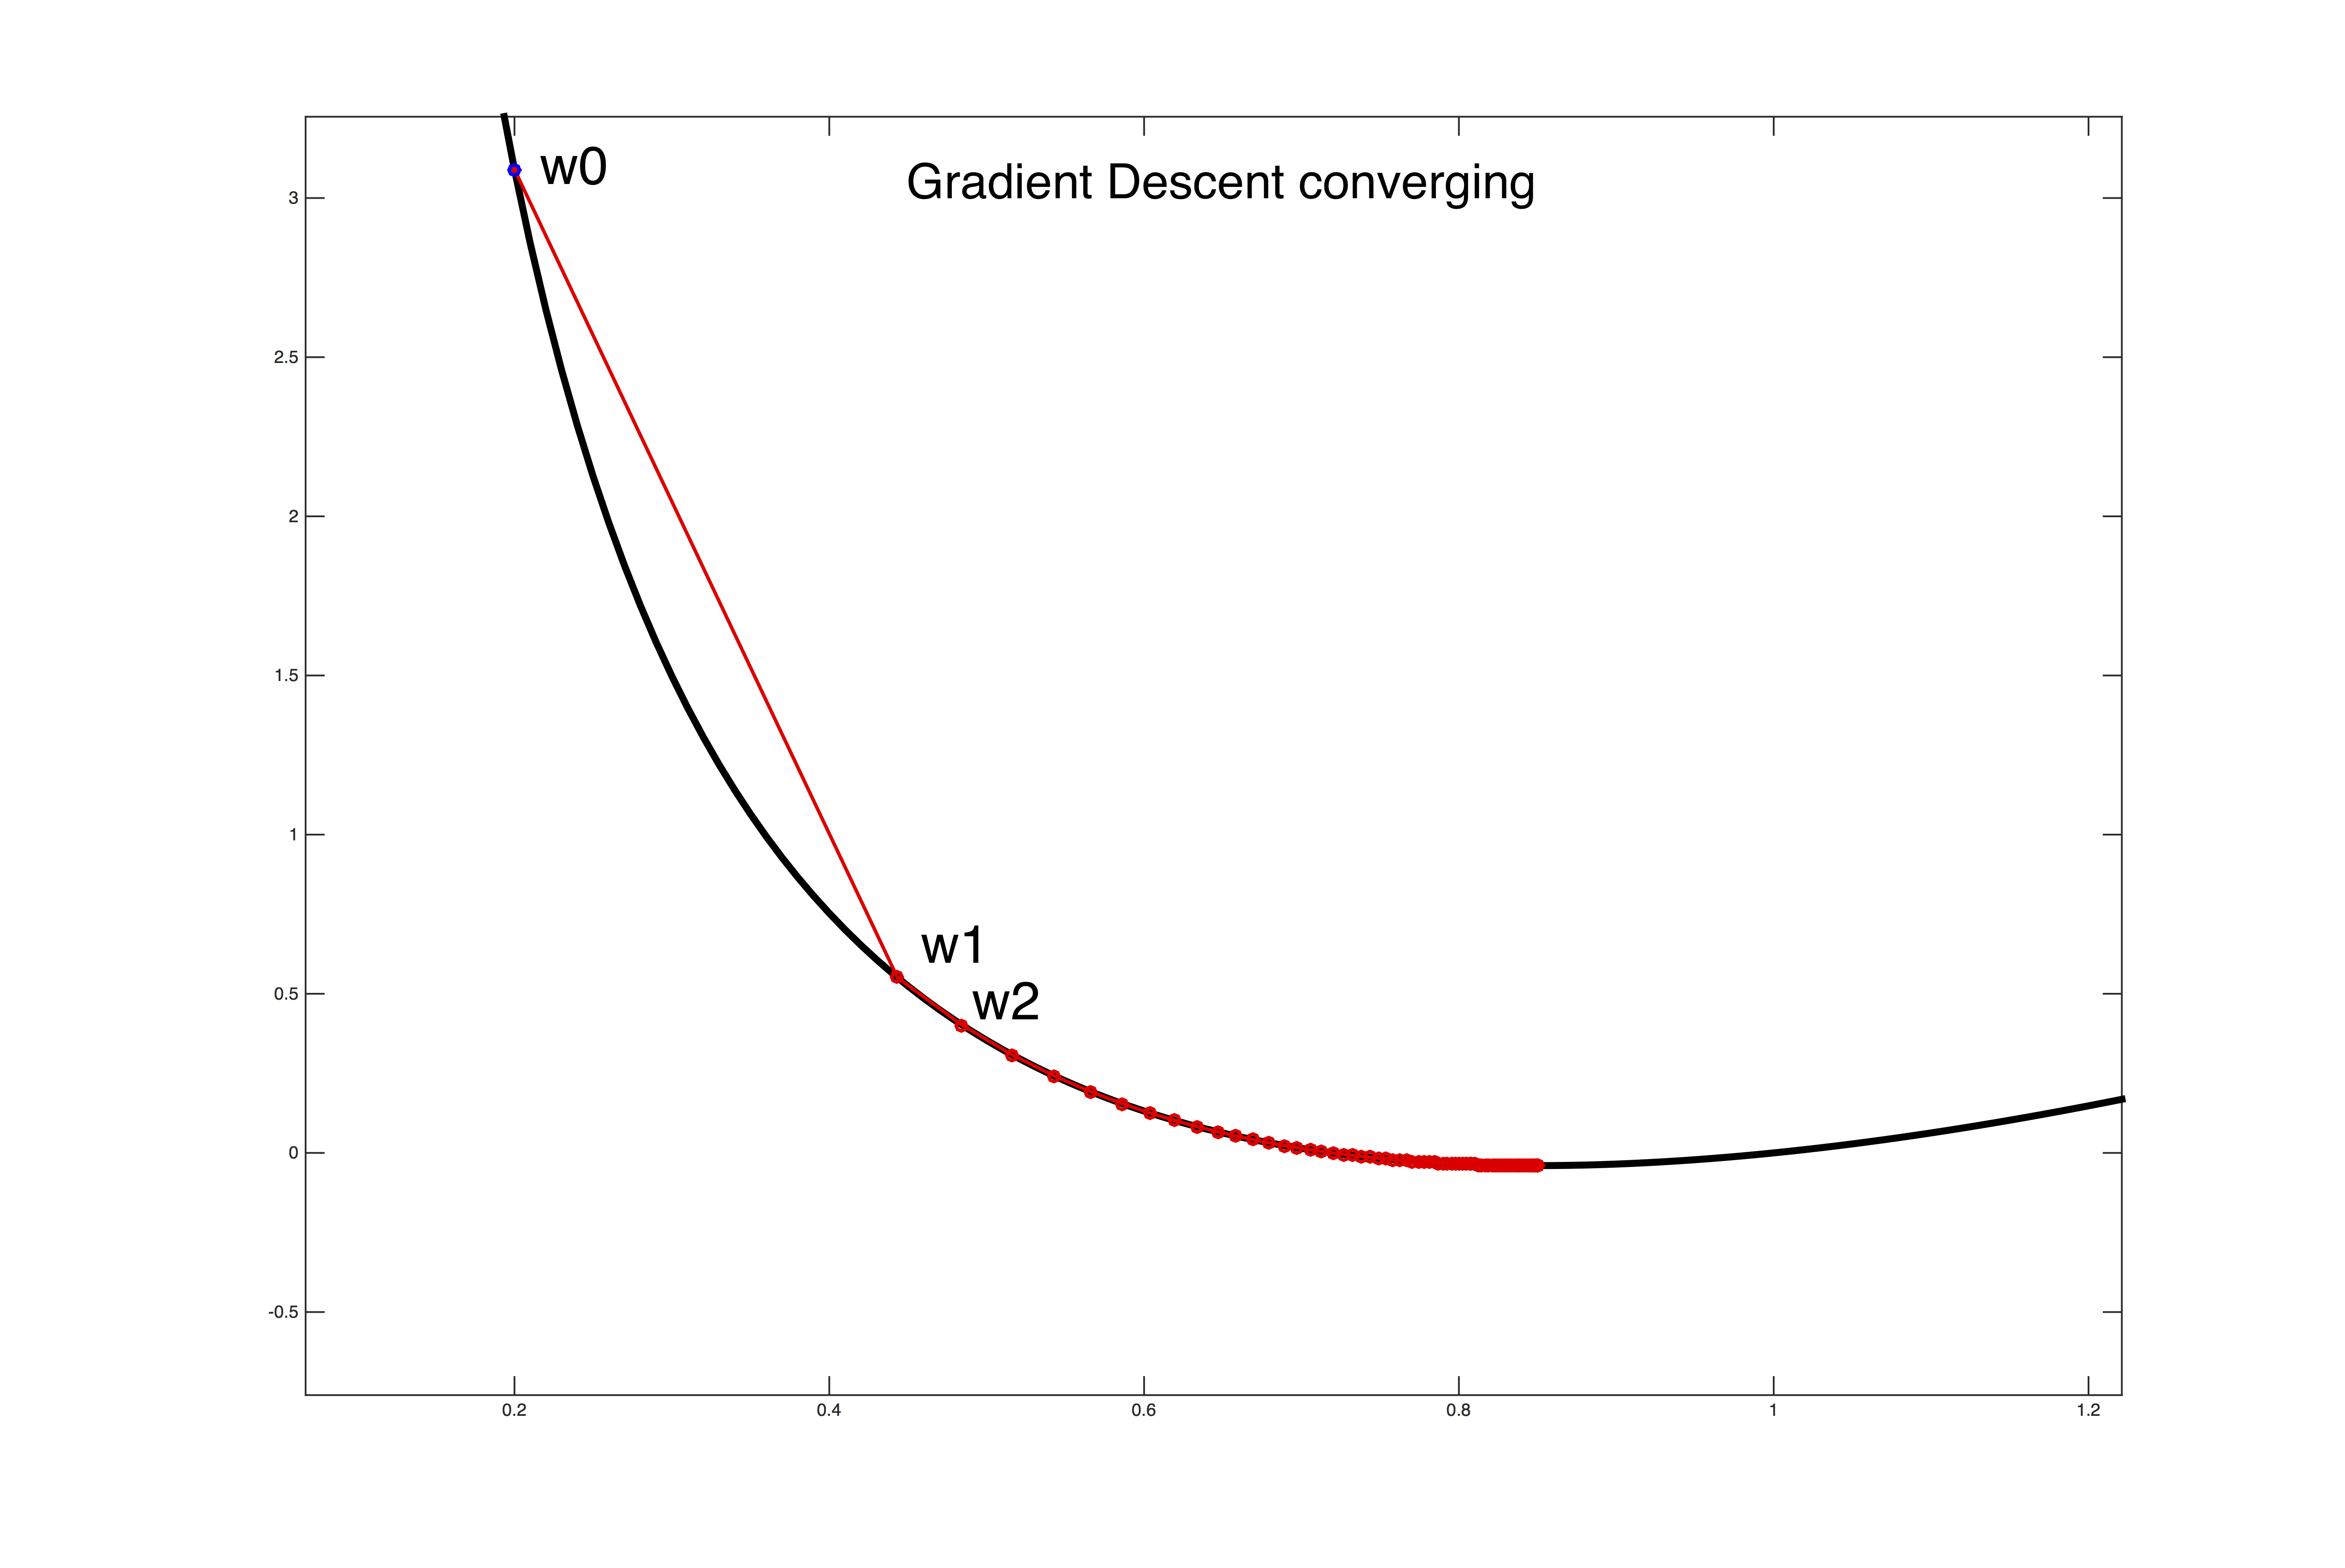
\includegraphics[width=8cm]{./Figs/lr_converge.jpg} }}%
    \qquad
    \subfloat[\centering $\alpha$ is too large]{{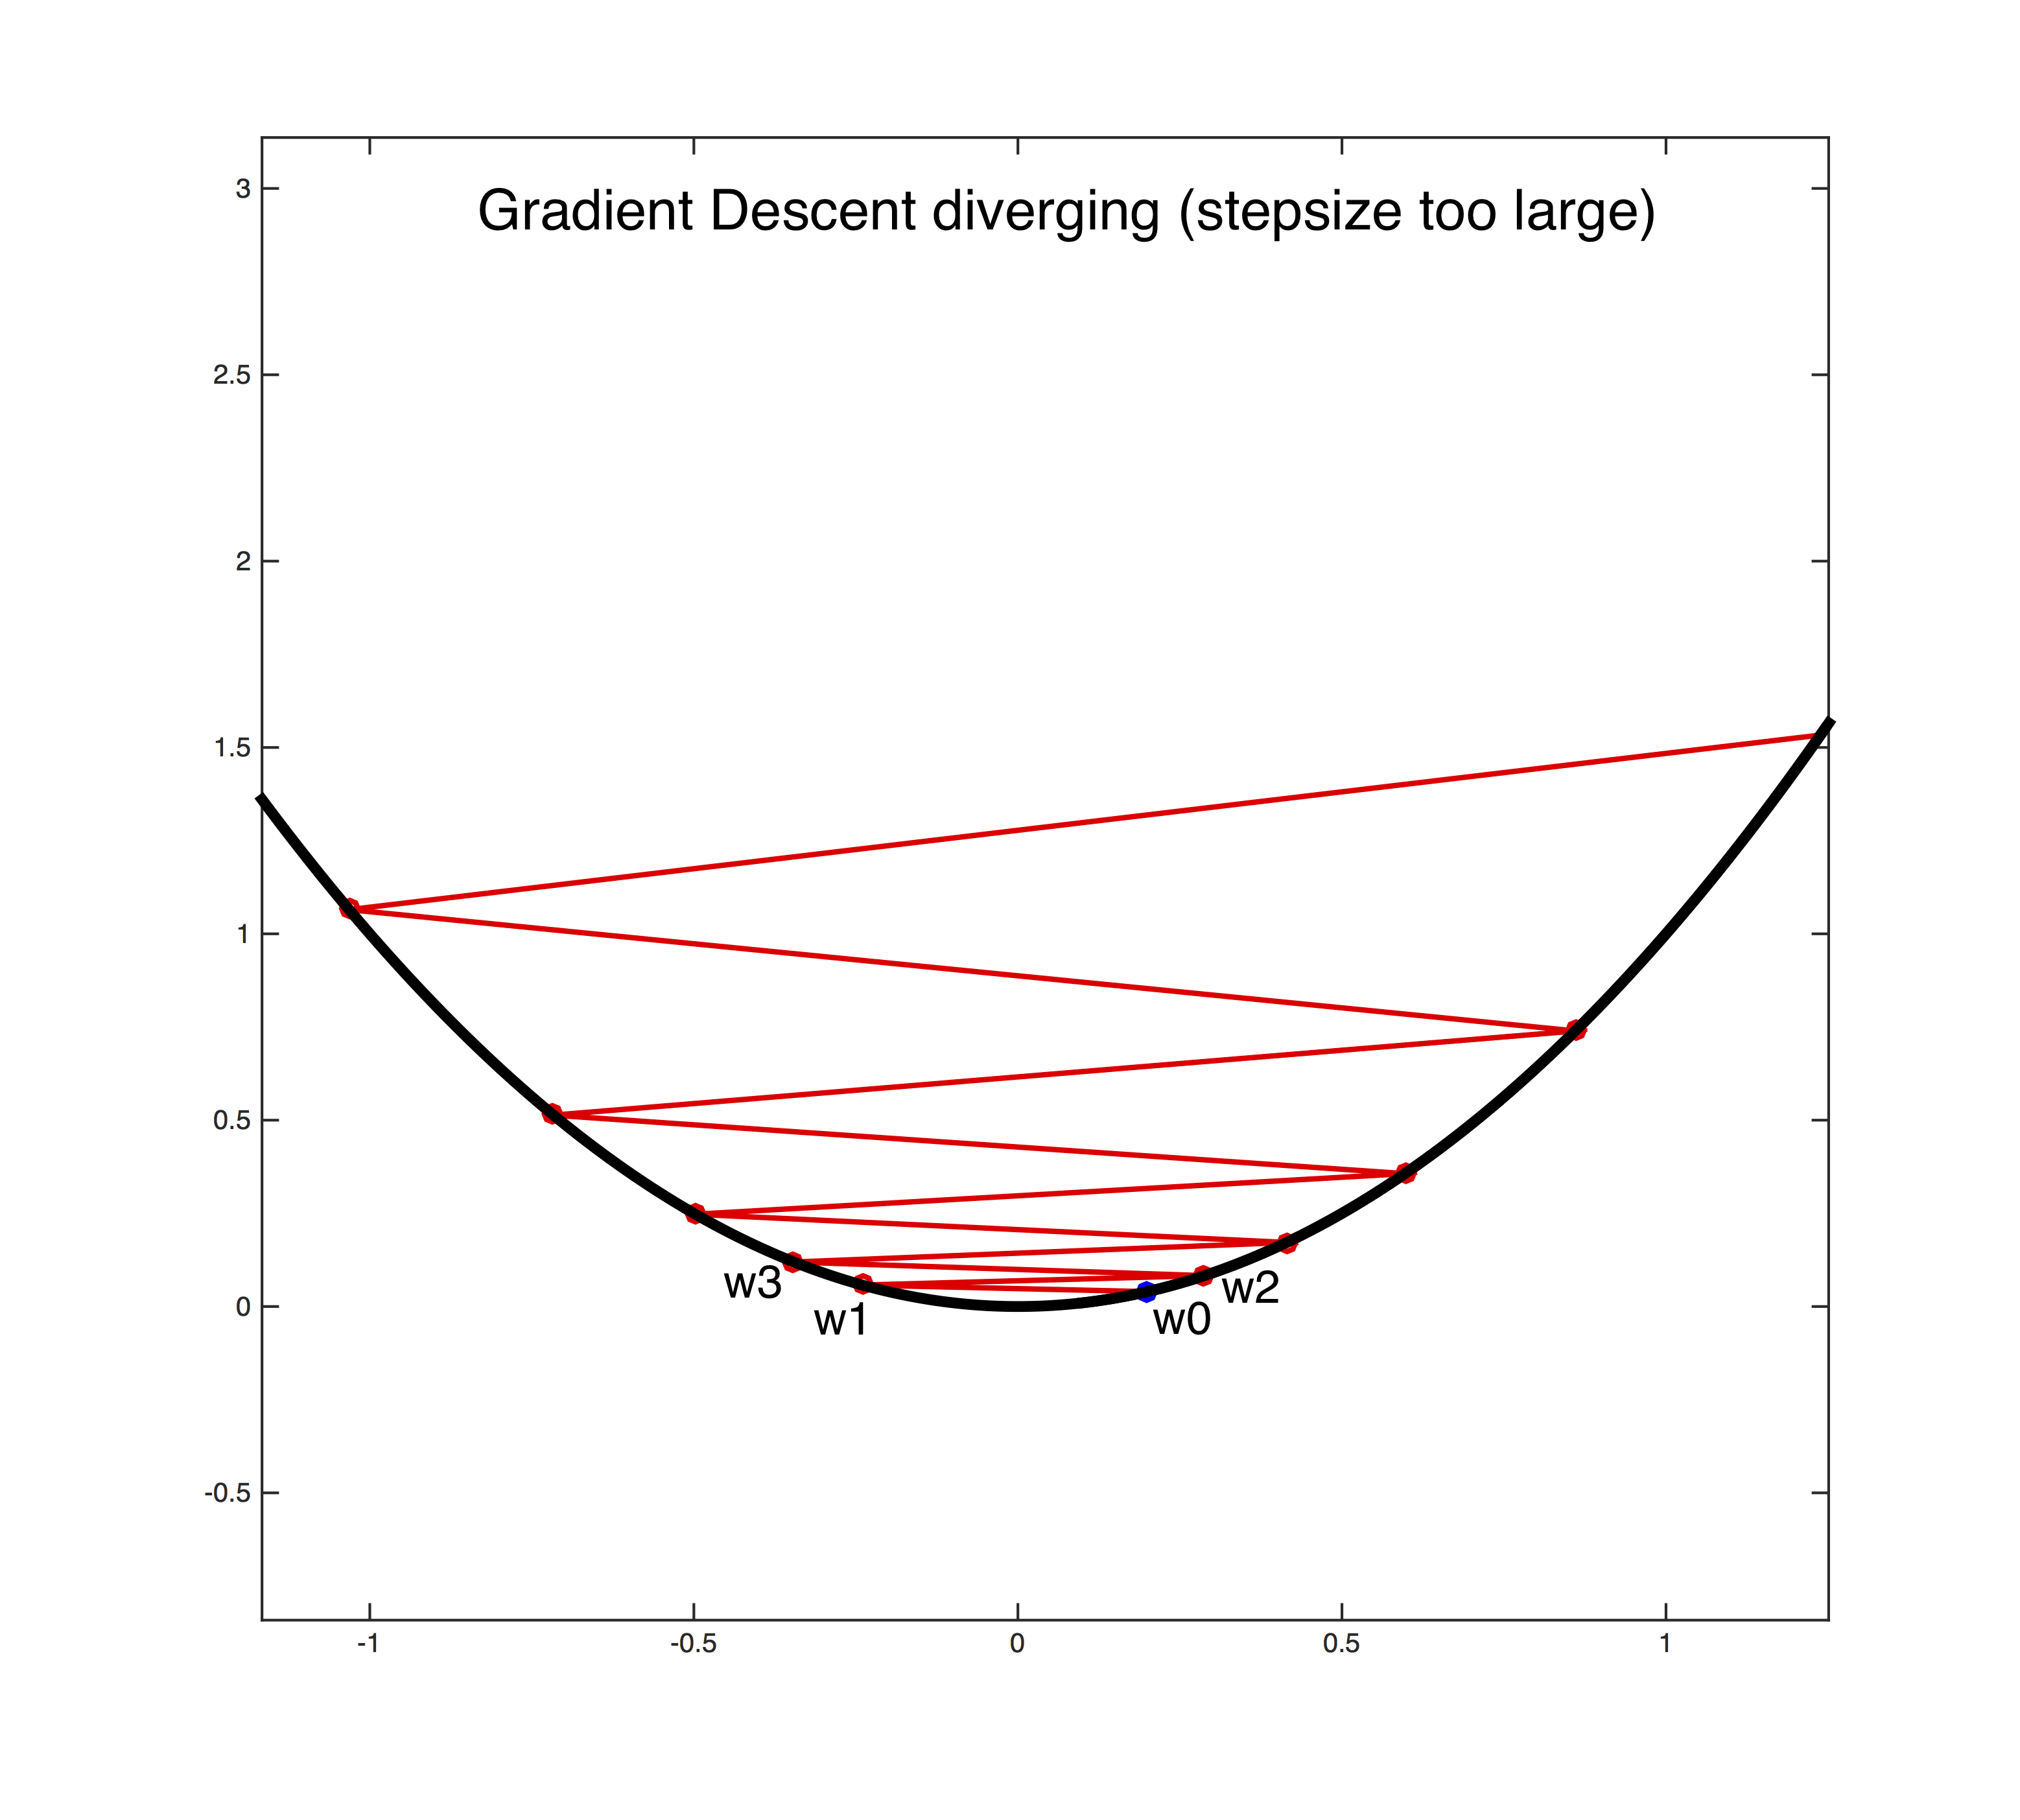
\includegraphics[width=7cm]{./Figs/lr_diverge.jpg} }}%
    \caption{Consequence of choosing $\alpha$, [Cornell CS4780, Lecture 7, Fall 2018]}%
    \label{fig:example}%
\end{figure}

% \subsection{\hl{Gradient with Respect to Weight}}
% Note that to change the output $\hat{y}$, we can only change the parameters $W$ and $b$. Therefore, we are interested in the gradient with respect to both these parameters:

\end{document}
